\documentclass[10pt,journal]{IEEEtran}
% Add the compsocconf option for Computer Society conferences.
\usepackage{mathtools}
\usepackage{amssymb,amsmath}
\usepackage[T1]{fontenc}
\usepackage{ifpdf}
\usepackage{url}
\ifpdf
\usepackage[pdftex]{graphicx}
\graphicspath{{figs/}}
\DeclareGraphicsExtensions{.pdf,.png,.jpg}
\else
\usepackage[dvips]{graphicx}

\graphicspath{{eps/}}
\DeclareGraphicsExtensions{.eps}
\fi
\usepackage{float}
%\usepackage[caption=false,font=footnotesize]{subfig}
\usepackage[font=footnotesize]{caption}
\usepackage{subcaption}
\usepackage{setspace}
\usepackage{balance}
\pdfminorversion=6
\hyphenation{op-tical net-works semi-conduc-tor}
\newcommand{\indentitem}{\setlength\itemindent{0pt}}
\usepackage{algorithmic}
\usepackage{algorithm}
\newcommand{\algorithmicinput}{\textbf{Input:}}
\newcommand{\INPUT}{\item[\algorithmicinput]}
\newcommand{\algorithmicoutput}{\textbf{Output:}}
\newcommand{\OUTPUT}{\item[\algorithmicoutput]}
\renewcommand{\algorithmicrequire}{\textbf{Pre Condition:}}
\renewcommand{\algorithmicensure}{\textbf{Post Condition:}}
\floatname{algorithm}{Procedure}
\usepackage{tikz}
\usetikzlibrary{matrix,arrows,circuits.ee,circuits.ee.IEC,shapes.geometric,shapes.misc}
\newcommand{\iap}{\textit{DREMS}}
%\newcommand{\iapfull}{\textbf{D}istributed \textbf{S}oftware \textbf{P}latform }
\newcommand{\iapfull}{\textbf{D}istributed \textbf{RE}altime \textbf{M}anaged \textbf{S}ystem}% Algorithmic modifications
\newcommand{\ALOOP}[1]{\ALC@it\algorithmicloop\ #1%
  \begin{ALC@loop}}
\newcommand{\ENDALOOP}{\end{ALC@loop}\ALC@it\algorithmicendloop}
\renewcommand{\algorithmicrequire}{\textbf{Input:}}
\renewcommand{\algorithmicensure}{\textbf{Output:}}
\newcommand{\algorithmicbreak}{\textbf{break}}
\newcommand{\BREAK}{\STATE \algorithmicbreak}
\newenvironment{noindlist}
 {\begin{list}{\labelitemi}{\leftmargin=0.1em \itemindent=0em \itemsep=0.3em}}
 {\end{list}}
\usepackage{multirow}

\begin{document}
\title{ DREMS-OS: An Operating System for Managed Distributed Real-time Embedded Systems }
\vspace{-0.1in}
\author{\IEEEauthorblockN{Abhishek Dubey, Gabor Karsai, Aniruddha Gokhale, William Emfinger, Pranav Kumar\\} 
\IEEEauthorblockA{
  ISIS, Dept of EECS, Vanderbilt University, Nashville, TN 37235, USA \\
 % Email:\{tbd@isis.vanderbilt.edu\}
}
}

% make the title area

%\setcounter{page}{1}
\maketitle
  In this paper, we explore the connection between secret key agreement and secure omniscience within the setting of the multiterminal source model with a wiretapper who has side information. While the secret key agreement problem considers the generation of a maximum-rate secret key through public discussion, the secure omniscience problem is concerned with communication protocols for omniscience that minimize the rate of information leakage to the wiretapper. The starting point of our work is a lower bound on the minimum leakage rate for omniscience, $\rl$, in terms of the wiretap secret key capacity, $\wskc$. Our interest is in identifying broad classes of sources for which this lower bound is met with equality, in which case we say that there is a duality between secure omniscience and secret key agreement. We show that this duality holds in the case of certain finite linear source (FLS) models, such as two-terminal FLS models and pairwise independent network models on trees with a linear wiretapper. Duality also holds for any FLS model in which $\wskc$ is achieved by a perfect linear secret key agreement scheme. We conjecture that the duality in fact holds unconditionally for any FLS model. On the negative side, we give an example of a (non-FLS) source model for which duality does not hold if we limit ourselves to communication-for-omniscience protocols with at most two (interactive) communications.  We also address the secure function computation problem and explore the connection between the minimum leakage rate for computing a function and the wiretap secret key capacity.
  
%   Finally, we demonstrate the usefulness of our lower bound on $\rl$ by using it to derive equivalent conditions for the positivity of $\wskc$ in the multiterminal model. This extends a recent result of Gohari, G\"{u}nl\"{u} and Kramer (2020) obtained for the two-user setting.
  
   
%   In this paper, we study the problem of secret key generation through an omniscience achieving communication that minimizes the 
%   leakage rate to a wiretapper who has side information in the setting of multiterminal source model.  We explore this problem by deriving a lower bound on the wiretap secret key capacity $\wskc$ in terms of the minimum leakage rate for omniscience, $\rl$. 
%   %The former quantity is defined to be the maximum secret key rate achievable, and the latter one is defined as the minimum possible leakage rate about the source through an omniscience scheme to a wiretapper. 
%   The main focus of our work is the characterization of the sources for which the lower bound holds with equality \textemdash it is referred to as a duality between secure omniscience and wiretap secret key agreement. For general source models, we show that duality need not hold if we limit to the communication protocols with at most two (interactive) communications. In the case when there is no restriction on the number of communications, whether the duality holds or not is still unknown. However, we resolve this question affirmatively for two-user finite linear sources (FLS) and pairwise independent networks (PIN) defined on trees, a subclass of FLS. Moreover, for these sources, we give a single-letter expression for $\wskc$. Furthermore, in the direction of proving the conjecture that duality holds for all FLS, we show that if $\wskc$ is achieved by a \emph{perfect} secret key agreement scheme for FLS then the duality must hold. All these results mount up the evidence in favor of the conjecture on FLS. Moreover, we demonstrate the usefulness of our lower bound on $\wskc$ in terms of $\rl$ by deriving some equivalent conditions on the positivity of secret key capacity for multiterminal source model. Our result indeed extends the work of Gohari, G\"{u}nl\"{u} and Kramer in two-user case.

% !TEX root = ../arxiv.tex

Unsupervised domain adaptation (UDA) is a variant of semi-supervised learning \cite{blum1998combining}, where the available unlabelled data comes from a different distribution than the annotated dataset \cite{Ben-DavidBCP06}.
A case in point is to exploit synthetic data, where annotation is more accessible compared to the costly labelling of real-world images \cite{RichterVRK16,RosSMVL16}.
Along with some success in addressing UDA for semantic segmentation \cite{TsaiHSS0C18,VuJBCP19,0001S20,ZouYKW18}, the developed methods are growing increasingly sophisticated and often combine style transfer networks, adversarial training or network ensembles \cite{KimB20a,LiYV19,TsaiSSC19,Yang_2020_ECCV}.
This increase in model complexity impedes reproducibility, potentially slowing further progress.

In this work, we propose a UDA framework reaching state-of-the-art segmentation accuracy (measured by the Intersection-over-Union, IoU) without incurring substantial training efforts.
Toward this goal, we adopt a simple semi-supervised approach, \emph{self-training} \cite{ChenWB11,lee2013pseudo,ZouYKW18}, used in recent works only in conjunction with adversarial training or network ensembles \cite{ChoiKK19,KimB20a,Mei_2020_ECCV,Wang_2020_ECCV,0001S20,Zheng_2020_IJCV,ZhengY20}.
By contrast, we use self-training \emph{standalone}.
Compared to previous self-training methods \cite{ChenLCCCZAS20,Li_2020_ECCV,subhani2020learning,ZouYKW18,ZouYLKW19}, our approach also sidesteps the inconvenience of multiple training rounds, as they often require expert intervention between consecutive rounds.
We train our model using co-evolving pseudo labels end-to-end without such need.

\begin{figure}[t]%
    \centering
    \def\svgwidth{\linewidth}
    \input{figures/preview/bars.pdf_tex}
    \caption{\textbf{Results preview.} Unlike much recent work that combines multiple training paradigms, such as adversarial training and style transfer, our approach retains the modest single-round training complexity of self-training, yet improves the state of the art for adapting semantic segmentation by a significant margin.}
    \label{fig:preview}
\end{figure}

Our method leverages the ubiquitous \emph{data augmentation} techniques from fully supervised learning \cite{deeplabv3plus2018,ZhaoSQWJ17}: photometric jitter, flipping and multi-scale cropping.
We enforce \emph{consistency} of the semantic maps produced by the model across these image perturbations.
The following assumption formalises the key premise:

\myparagraph{Assumption 1.}
Let $f: \mathcal{I} \rightarrow \mathcal{M}$ represent a pixelwise mapping from images $\mathcal{I}$ to semantic output $\mathcal{M}$.
Denote $\rho_{\bm{\epsilon}}: \mathcal{I} \rightarrow \mathcal{I}$ a photometric image transform and, similarly, $\tau_{\bm{\epsilon}'}: \mathcal{I} \rightarrow \mathcal{I}$ a spatial similarity transformation, where $\bm{\epsilon},\bm{\epsilon}'\sim p(\cdot)$ are control variables following some pre-defined density (\eg, $p \equiv \mathcal{N}(0, 1)$).
Then, for any image $I \in \mathcal{I}$, $f$ is \emph{invariant} under $\rho_{\bm{\epsilon}}$ and \emph{equivariant} under $\tau_{\bm{\epsilon}'}$, \ie~$f(\rho_{\bm{\epsilon}}(I)) = f(I)$ and $f(\tau_{\bm{\epsilon}'}(I)) = \tau_{\bm{\epsilon}'}(f(I))$.

\smallskip
\noindent Next, we introduce a training framework using a \emph{momentum network} -- a slowly advancing copy of the original model.
The momentum network provides stable, yet recent targets for model updates, as opposed to the fixed supervision in model distillation \cite{Chen0G18,Zheng_2020_IJCV,ZhengY20}.
We also re-visit the problem of long-tail recognition in the context of generating pseudo labels for self-supervision.
In particular, we maintain an \emph{exponentially moving class prior} used to discount the confidence thresholds for those classes with few samples and increase their relative contribution to the training loss.
Our framework is simple to train, adds moderate computational overhead compared to a fully supervised setup, yet sets a new state of the art on established benchmarks (\cf \cref{fig:preview}).


\section{Related work}\label{sect:related}

\paragraph{{Recovery}} {The works most closely most closely related to ours are those based on the \emph{recovery} notion, that is, the type system of Gordon et al. \cite{GordonEtAl12} and the Pony language  \cite{ClebschEtAl15}.} Indeed, the capsule property has many variants in the literature, such as \emph{isolated} \cite{GordonEtAl12}, \emph{uniqueness} \cite{Boyland10} and \emph{external uniqueness}~\cite{ClarkeWrigstad03}, \emph{balloon} \cite{Almeida97,ServettoEtAl13a}, \emph{island} \cite{DietlEtAl07}. 
%The fact that aliasing can be controlled by using \emph{lent} (\emph{borrowed}) references is well-known~\cite{Boyland01,NadenEtAl12}.
However, before the work of Gordon et al. \cite{GordonEtAl12}, the capsule property was only ensured in simple situations, such as using a primitive deep clone operator, or composing subexpressions with the same property.

The important novelty of the type system of Gordon et al. \cite{GordonEtAl12} has been \emph{recovery}, that is, the ability to ensure properties (e.g., capsule or immutability) by keeping into account not only the expression itself but the way the surrounding context is used. {Notably,} an expression which does not use external mutable references is recognized to be a capsule. 
{In the Pony language \cite{ClebschEtAl15}  the ideas of Gordon et al. \cite{GordonEtAl12} are extended to a richer set of reference immutability permissions. In their terminology \texttt{value} is immutable, \texttt{ref} is mutable, \texttt{box} is similar to \emph{readonly} as often found in literature, different from our $\readable$ since it can be aliased. An ephemeral isolated reference \lstinline{iso^} is similar to a $\capsule$ reference in our calculus, whereas non ephemeral \texttt{iso} references offer destructive reads and are more
similar to isolated fields \cite{GordonEtAl12}. Finally, \texttt{tag} only allows object identity checks and \texttt{trn} (transition) is a subtype of \texttt{box} that can be converted to \texttt{value}, providing a way to create values without using isolated references. The last two qualifiers have no equivalent in our
work or in  \cite{GordonEtAl12}.}

Our {type system greatly enhances the recovery mechanism used in such previous work \cite{GordonEtAl12,ClebschEtAl15} by using lent references, and rules \rn{t-swap} and \rn{t-unrst}.} For instance, the examples in \refToFigure{TypingOne} and \refToFigure{TypingTwo} would be ill-typed in \cite{GordonEtAl12}. 

{A minor difference with the type systems of Gordon et al. \cite{GordonEtAl12} and Pony \cite{GordonEtAl12,ClebschEtAl15} is that we only allow fields to be $\mutable$ or $\imm$.
Allowing \emph{readonly} fields means holding a reference that is useful for observing but non making remote modifications. However, our type system supports the $\readable$ modifier rather than the \emph{readonly}, and the $\readable$ qualifier includes the $\lent$ restriction. Since something which is $\lent$ cannot be saved as part of a $\mutable$ object, $\lent$ fields are not compatible with the current design where objects are born $\mutable$. The motivation for supporting $\readable$ rather than \emph{readonly} is discussed in a specific point later.
Allowing $\capsule$ fields means that programs can store an externally unique object graph into the heap and decide later whether to unpack
 permanently or freeze the reachable objects.  This can be useful, but, as for $\readable$ versus \emph{readonly}, our opinion is that this power is hard to use for good, since
it requires destructive reads, as discussed in a specific point later. 
In most cases, the same expressive power can be achieved by having the
field as $\mutable$ and recovering the $\capsule$ property for the outer object.}

\paragraph{Capabilities}
 {In other proposals \cite{HallerOdersky10,CastegrenWrigstad16} types are compositions of one or more \emph{capabilities}. The modes of the capabilities in a type control how resources of that
type can be aliased. The compositional aspect of capabilities is an important difference
from type qualifiers, as accessing different parts of an object through different capabilities in the same type gives different properties. 
By using capabilities it is possible to obtain an expressivity which looks similar to our type system, even though with different sharing notions and syntactic constructs. For instance, the \emph{full encapsulation} notion in \cite{HallerOdersky10}\footnote{{This paper includes a very good survey of work in this area, notably explaining the difference between \emph{external uniqueness}~\cite{ClarkeWrigstad03} and \emph{full encapsulation}.}}, apart from the fact that sharing of immutable objects is not allowed, is equivalent to the guarantee of our $\capsule$ qualifier, while
our $\lent$ and their \Q|@transient| achieve similar results in different ways.}
Their model has a higher syntactic/logic overhead to explicitly  track regions.
As for all work before~\cite{GordonEtAl12}, objects need to be born \Q|@unique| and the type system 
permits to manipulate data preserving their uniqueness. With recovery~\cite{GordonEtAl12},
instead, we can forget about uniqueness, use normal code designed to work on conventional shared data, and then
recover the aliasing encapsulation property.

\paragraph{Destructive reads} Uniqueness can be enforced by destructive reads, i.e., assigning a copy of 
the unique reference to a variable an destroying the original reference, see
\cite{GordonEtAl12,Boyland10}. Traditionally, borrowing/fractional permissions~\cite{NadenEtAl12} are related to uniqueness  in the opposite way: a unique reference can be borrowed,
it is possible to track when all borrowed aliases are buried~\cite{Boyland01}, and then uniqueness can be recovered.
These techniques offers a sophisticate alternative to destructive reads. 
We also wish to avoid destructive reads. In our work, we ensure uniqueness by linearity, that is, by allowing at most
one use of a $\capsule$ reference.

In our opinion, programming with destructive reads is involved and hurts the correctness of the program, since it leads to the style of programming outlined below, where \Q@a.f@ is a unique/isolated field with destructive read.
\begin{lstlisting}
a.f=c.doStuff(a.f)//style suggested by destructive reads
\end{lstlisting}
The object referenced by \lstinline{a}{} has an \emph{unique/isolated} field \lstinline{f} containing an object \lstinline{b}.
This object \lstinline{b}{} is passed to a client \lstinline{c}{}, which can use (potentially modifying) it. A typical pattern is that the result of such computation is a reference to \lstinline{b}{}, which \lstinline{a}{} can then recover. This approach allows \emph{isolated} fields, as shown above, but has  a serious drawback:
an \emph{isolated} field can become unexpectedly not available (in the example, during execution of \lstinline{doStuff}{}), hence any object contract
involving such field can be broken.
{This can cause {subtle} bugs if \Q@a@ is in the reachable object graph of \Q@c@.}

In our approach, the  $\capsule$ qualifier cannot be applied to fields. Indeed, the ``only once'' use of capsule variables 
makes no sense on fields.
{However, we support the same level of control of the reachable object graph by passing mutable objects to clients as $\lent$, in order to control aliasing behaviour.
That is, the previous code can be rewritten} as follows:
\begin{lstlisting}
c.doStuff(a.f())//our suggested style
\end{lstlisting}
{where \Q@a.f()@ is a getter returning the field as $\lent$.
Note how, during the execution of \Q@doStuff@, \Q@a.f()@ is still available, and,} after the execution of \Q@doStuff@, the aliasing relation {for this field is the same as it was
before \Q@doStuff@ was called.}

\paragraph{Ownership} A {closely related} stream of research is that on \emph{ownership} (see an overview in~\cite{ClarkeEtAl13}) which, however, offers an {opposite} approach. In the ownership approach, it is provided a way to express and prove the ownership invariant\footnote{{Ownership invariant (owner-as-dominator):
Object $o_1$ is owned by object  $o_2$ if in the object graph $o_2$
is a dominator node for $o_1$;
that is, all paths from the roots of the graph (the stack variables)
to $o_1$ pass throw $o_2$.
Ownership invariant (owner-as-modifier):
Object $o_1$ is owned by object  $o_2$ if any field update over $o_1$
is initiated by $o_2$, that is, a call of a method of $o_2$ is present
in the stack trace.}}, which, however, is expected to be guaranteed by defensive cloning, as explained below. In our approach, instead, the capsule concept models an efficient \emph{ownership transfer}. In other words, when an object $\x$ is ``owned'' by another object $\y$, it remains always true that $\y$ can be only accessed only through $\x$, whereas the capsule notion is more dynamic: a capsule can be ``opened'', that is, assigned to a standard reference and modified, and then we can recover the original capsule guarantee. 

For example, assuming a graph with a list of nodes, and a constructor taking in input such list,
the following code establishes the ownership invariant using $\capsule$, and ensures that it cannot be violated using $\lent$.
\begin{lstlisting}
class Graph{
  private final NodeList nodes;
  private Graph(NodeList nodes){this.nodes=nodes; }

  static Graph factory(capsule NodeList nodes){
    return new Graph(nodes);
    }
  
  lent NodeList borrowNodes(mut){return nodes;}
}
\end{lstlisting}
Requiring the parameter of the \lstinline{factory}{} method to be a $\capsule$ guarantees that the list of nodes provided as argument is not referred from the external environment. 
The factory \emph{moves} an isolated portion of store as local store of the newly created object. 
Cloning, if needed, becomes responsibility of the client which provides the list of nodes to the graph. The getter tailors the exposure level of the private store. 

Without aliasing control ($\capsule$ qualifier),  in order to ensure ownership of its list of nodes, the {factory method} should clone the argument, since it comes from an external client environment.
This solution, called  \label{cloning} \emph{defensive cloning}~\cite{Bloch08}, is very popular in the Java community, but inefficient,
since it requires to duplicate the reachable object
graph of the parameter, until immutable nodes are
reached.\footnote{{In most languages, for owner-as-modifier defensive cloning is needed
only when new data is saved inside of an object, while for owner-as-dominator it is needed also when internal data are exposed.}}
Indeed, many programmers prefer to write {unsafe}
 code instead of using defensive cloning for efficiency reasons.
However, this unsafe approach is only possible when programmers have control of the client code, that is, they are not 
working in a library setting.
Indeed many important Java libraries (including the standard Java libraries) today
use defensive cloning to ensure ownership of their internal state.

As mentioned above, our approach is the opposite of the one offered by many ownership approaches, which provide a formal way to express  and prove the ownership invariant that, however, are expected to be guaranteed by defensive cloning. 
We, instead, model an efficient \emph{ownership transfer} through the capsule concept, then, 
duplication of memory, if needed, is performed on the client side\footnote{
Other work in literature supports ownership transfer, see for example~\cite{MullerRudich07, ClarkeWrigstad03}.
In literature it is however applied to uniquess/external uniqueness, thus not {the whole} reachable object graph is transfered.
}.

Moreover, depending on how we expose the owned data, we can closely model
both \emph{owners-as-dominators} (by providing no getter)
and \emph{owners-as-qualifiers} (by providing a \Q@read@ getter). In the example, the method \lstinline{borrowNodes}{} is an example of a $\lent$ getter, a third variant besides the two described on page \pageref{exposer}.  This variant is particularly useful in the case of a field which is owned, indeed, \Q@Graph@ instances can release the mutation control of their nodes without permanently {losing} the aliasing control.

In our approach all properties are deep. On the opposite side, most ownership approaches allows one to distinguish
subparts of the reachable object graph that are referred but not logically owned. This viewpoint has many advantages, for example the Rust language\footnote{\texttt{rust-lang.org}} leverages on ownership to control object deallocation without a garbage collector.
Rust employs a form of uniqueness that can be seen as a restricted ``owners-as-dominators" discipline.  
Rust lifetime parameters behave like additional ownership parameters~\cite{OstlundEtAl08}.

However, in most ownership based approaches 
it is not trivial to encode the concept of full encapsulation, while supporting (open) sub-typing and avoiding defensive cloning.
This depends on how any specific ownership approach entangles subtyping with 
 gaining extra ownership parameters
and extra references to global ownership domains.

\paragraph{Readable notion} Our $\readable$ qualifier is different from \emph{readonly} as used, e.g., in \cite{BirkaErnst04}.
 An object cannot be modified through a readable/readonly reference. However, 
$\readable$ also prevents aliasing.
As discussed in \cite{Boyland06}, readonly semantics can be easily misunderstood by
programmers. Indeed, some wrongly believe it means immutable, whereas the object denoted by a readonly reference can be modified through other references, while others do not realize that readonly data can still be saved in fields, and thus used as a secondary window to observe the change in the object state.
Our proposal addresses both problems, since we explicitly support the $\imm$ qualifier, hence it is more difficult for programmers to confuse the two concepts, and our $\readable$ (readonly + lent) data  cannot be saved in client's fields.

Javari~\cite{TschantzErnst05} also supports the \emph{readonly} type qualifier, and makes a huge design effort to support \emph{assignable} and \emph{mutable} fields, to have fine-grained readonly constraints.  The need of such flexibility is motivated by performance reasons.
In our design philosophy, we do not offer any way of breaking the invariants enforced by the type system. Since our invariants are very strong, we expect compilers to be able to perform optimization, thus recovering most of the efficiency lost to properly use immutable and readable objects.




% $Id: taskModel.tex 3909 2013-10-22 06:07:02Z dabhishe $
\vspace{-0.09in}
\section{DREMS Architecture}
\label{sec:task_model}
% This section provides background material and states assumptions for the rest of the paper. 
% in this paper. 
% We also describe the underlying
%system model used for our research.
%\vspace{-0.05in}
%\subsection{\iap\ Architecture}
\iap\ \cite{ISIS_F6_Aerospace:12,6899124,4813} is a distributed system architecture that consists
of one or more computing nodes grouped into a cluster. It is conceptually similar to the recent Fog Computing Architecture \cite{vaquero2014finding}. Distributed applications, composed from cooperating
processes called \textit{actors}, provide services for the end-user.
Actors specialize the notion of OS processes; 
they have persistent identity that allows them to be transparently
migrated between nodes, and they have strict limits on resources that
they can use.  Each actor is constructed from one or more reusable
components~\cite{ISIS_F6_ISORC:13,4813} where each component is
single-threaded.  
% Abhishek, commenting this out.
% Recently, this architecture has been extended to create  applications for smart grid \cite{4813}. 

% \vspace{-0.05in}
% \subsection{The Linux Scheduler}
% \label{sec:linuxScheduler}
% The \iap\ OS scheduler builts upon the standard Linux scheduler
% (kernel version: 3.2.7).  The scheduler is responsible for allocating
% CPU resource(s) to all currently running computational entities.
% Schedulers are implemented in the Linux kernel through \emph{scheduler
%   classes}.  The two important scheduler classes are CFS (Completely Fair
% Scheduler) and the RT (Real Time) scheduler~\cite{mauerer2008}.
% The CFS scheduler attempts to allocate CPU time between processes
% fairly, while the RT scheduler selects processes based on their priority. 

% Tasks eligible for scheduling are maintained in a structure called the
% \emph{runqueue}. Each CPU core has its own runqueue. However
% the runqueue is not necessarily just a queue: it consists of a 
% %-- it is a container using a data structure that contains 
% a bit array,  with one bit for each priority level and a list containing the 
% tasks ready to be scheduled at that level.
% The bit at a level is set to one when there are tasks at that level.
% A 0 value indicates an empty queue at that level. In a multi core
% system, this structure is replicated per CPU. In a fully preemptive
% mode, the scheduling decision is made by  evaluating which task should be
% executed next on a CPU when an interrupt handler exits, when a 
% system call returns, or when the scheduler function is
% explicitly invoked to preempt the current process.

%\begin{figure}[t]
%\centering
%\includegraphics[width=0.45\textwidth]{runqueue}
%\caption{Scheduler Runqueues}
%\label{fig:runqueue}
%\end{figure}

\iffalse
Next sections describe the \iap\ Scheduler features and their main
algorithms. This scheduler was implemented by changing the behavior of
the linux scheduler described in this subsection.  
\fi
\vspace{-0.05in}
%\subsection{Spatial and Temporal Partitioning}
%\label{sec:tasks}

\iffalse
While most tasks\footnote{We use the term threads and tasks
  interchangeably in this paper.} perform application functions,
some tasks are used for system management and mission-critical functions.  
Thus, we group these tasks into different criticality levels: (a) 
\emph{Critical} tasks are those tasks which are required
for system and mission management; (b)
\emph{Application} tasks perform mission-specific, non-critical work; 
(c)
%\emph{System Management}[kernel] tasks provide the interfaces to the
%kernel resources and can be configured to have a fixed percentage of
%CPU time reserved for these tasks; and finally (d)
 \emph{Best Effort}
tasks are those low priority tasks that are scheduled only when there
are no runnable tasks from the previous two categories.
\fi 
\begin{figure}[t]
\centering
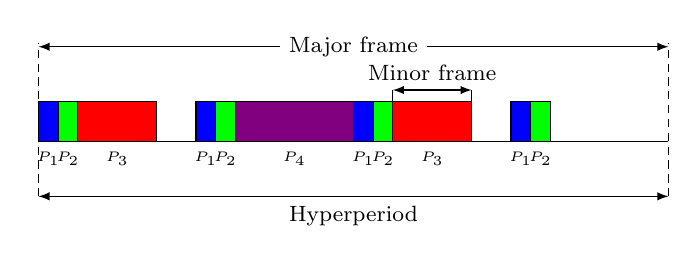
\begin{tikzpicture}[x=1cm,y=1cm, 
every label/.style={font=\tiny},
p1/.style={shape=rectangle,draw,fill=blue, align=center,font=\tiny,minimum height=5mm,minimum width=2.5mm},
p2/.style={shape=rectangle,draw,fill=green,align=center,font=\tiny,minimum height=5mm,minimum width=2.5mm},
p3/.style={shape=rectangle,draw,fill=red,  align=center,font=\tiny,minimum height=5mm,minimum width=10mm},
p4/.style={shape=rectangle,draw,fill=red!50!blue,align=center,font=\tiny,minimum height=5mm,minimum width=15mm},
]
\def\pdist{0.25}\def\hpy{-.95}\def\MF{.95}\def\mfh{.4}\def\mfbeg{17.5*\pdist}\def\mfend{21.5*\pdist}\def\labelpos{270}
\node[p1](P11) at (   0*\pdist,0) [label=\labelpos:$P_1$]{}; \node[p2](P21) at ( 1*\pdist,0) [label=\labelpos:$P_2$] {};
\node[p3](P31) at ( 3.5*\pdist,0) [label=\labelpos:$P_3$]{}; 
\node[p1](P12) at (   8*\pdist,0) [label=\labelpos:$P_1$]{}; \node[p2](P22) at ( 9*\pdist,0) [label=\labelpos:$P_2$] {};
\node[p4](P41) at (12.5*\pdist,0) [label=\labelpos:$P_4$]{}; 
\node[p1](P13) at (  16*\pdist,0) [label=\labelpos:$P_1$]{}; \node[p2](P23) at (17*\pdist,0) [label=\labelpos:$P_2$] {};
\node[p3](P32) at (19.5*\pdist,0) [label=\labelpos:$P_3$]{};
\node[p1](P14) at (  24*\pdist,0) [label=\labelpos:$P_1$]{}; \node[p2](P24) at (25*\pdist,0) [label=\labelpos:$P_2$] {};
\draw[densely dashed,-] (-0.5*\pdist,\hpy) -- (-0.5*\pdist,1); \draw[densely dashed,-] (31.5*\pdist,\hpy) -- (31.5*\pdist,1);
\draw[-] (-0.5*\pdist,-.25) -- (31.5*\pdist,-.25);
\draw[latex-latex] (-0.5*\pdist,\hpy) -- (31.5*\pdist,\hpy) node [below,align=center,midway,font=\footnotesize] {Hyperperiod};
\draw[latex-latex] (-0.5*\pdist,\MF) -- node[sloped,fill=white,font=\footnotesize]{Major frame} (31.5*\pdist,\MF);
%
\draw[-] (\mfbeg,0) -- (\mfbeg,\mfh); \draw[-] (\mfend,0) -- (\mfend,\mfh);
\draw[latex-latex] (\mfbeg,\mfh) -- (\mfend,\mfh) node [above,align=center,midway,font=\footnotesize] {Minor frame};
\end{tikzpicture}%

\caption{A Major Frame. The four partitions (period,duration) in this frame are $P_1$ (2s, 0.25s), $P_2$ (2s, 0.25s), $P_3$ (4s, 1s), and $P_4$ (8s, 1.5s). }
%where the first number is the period and the second number is the duration of the partition.}
\label{fig:validschedule}
\vspace{-0.2in}
\end{figure}

%The length of the repeating frame is also known as the \emph{major frame}.  

%Given a valid schedule as input, the
%scheduler guarantees that actors in separate temporal partitions
%cannot interfere with each other's CPU resource usage.  

%
%
%. For the RT scheduler it is an array combined with bits
%indicating priority. Tasks are added  to the runqueue when they are in ready state and are removed from the runqueue when they are waiting for either a reseource or are sleeping for some time. 
%
%
%
% and removed from the runqueue as they become ready or 
%
%
%The runqueues do not necessarily contain all the
%existing tasks in the system - only those which are eligible for
%scheduling. One example for tasks which are not in any of the queues
%are inactive tasks. When a task becomes inactive it is removed from
%the runqueues (\texttt{dequeue\_task}) and a timer is started. When the
%timer expires, the task is added back to the runqueue
%(\texttt{enqueue\_task}). This dequeuing and enqueing happens each
%time a task changes its state from ready to another state.
%
%When SMP (Symmetric Multiprocessing) is enabled, each CPU manages its own runqueue. Tasks are
%occasionally migrated between CPUs based on a balancing algorithm. The
%RT scheduler runqueue consists of a bitmap and a linked list for each
%priority level. The bitmap contains "1" if the given list contains any
%element - this allows the scheduler to jump to the highest priority 
%ready task in constant time. When a task is added to the list the
%bitmap is updated and the task is added to the linked list belonging
%to the given level. The same steps happen for task removal or a
%change in a task's priority. During a scheduling decision, the
%core scheduler goes through the scheduler classes in their priority
%order and calls the \texttt{pick\_next\_task} function. If it returns with a task, the task will get prioritized. 
%If no task is ready to run, the idle task is scheduled. A 
%scheduling decision happens in one of the following situations:
%
%\begin {itemize}
%\item [A)] When an interrupt handler exits (including the interrupt invoked
%  by the periodic tick timer).
%\item [B)] When a system call returns.
%\item [C)] When the scheduler is invoked explicitly by the current running
%  task.
%\end {itemize}

% TODO:  I presume this has yet to be done?
%{\bf describe the preemption-RT patch}



%!TEX root = main.tex
% $Id: f6sched.tex 3898 2013-10-22 04:52:42Z csanad $
%\section{\iap\ OS Scheduler}
%\label{sec:scheduler}
%This section delves into the details of the \iap\ OS scheduler and its
%capabilities.

\subsection{Partitioning Support}
\label{sec:scheduler}
The system guarantees spatial isolation between actors  by (a)
providing  a separate address space for each actor; (b) enforcing that an
I/O device can be accessed by only one actor at a time; and (c)
facilitating temporal isolation between processes by the scheduler.
Spatial isolation is implemented by the Memory Management Unit of the CPU,  
while temporal isolation is provided via ARINC-653~\cite{ARINC-653} style
\textit{temporal partitions}, implemented in the OS scheduler. 

%-- a periodically repeating fixed interval of the CPU's time exclusively assigned to a group of 
% cooperating actors of the same  application. 
% Abhishek, in the intro we have mentioned limitations with such a
% partitioning scheme and cited the very same reference. So here we need
% to say a sentence saying that there is a slight difference as
% explained in Section~\ref{sec:scheduler}.

A temporal partition is characterized by two parameters: period and
duration.  The period reflects how often the tasks of the
partition will be guaranteed CPU allocation.  The duration governs the
length of the CPU allocation window in each cycle.  Given the period
and duration of all temporal partitions, an execution schedule can be
generated by solving a series of constraints, see~\cite {ACM_SPE:10}.
A feasible solution, \emph{e.g.} Figure~\ref{fig:validschedule}, comprises
a repeating frame of windows, where each window is assigned to a
partition.  These windows are called \emph{minor frames}.  The length
of a window assigned to a partition is always the same as the duration
of that partition.  The repeating frame of minor frames, known as the \emph{major frame},
has a length called the \emph{hyperperiod}.  The hyperperiod is the lowest common multiple
of the partition periods.  


\subsection{Criticality Levels Supported by the \iap\ OS Scheduler}
\label{sec:criticality_levels}
The \iap\ OS scheduler can manage CPU's time
for tasks on three different criticality levels:
\emph{Critical}, \emph{Application} and \emph{Best Effort}.
The \emph{Critical} tasks provide kernel level services and system
management services. These tasks will be scheduled based on their
priority whenever they are ready. \emph{Application} tasks are
mission specific and are isolated from each other. These tasks are
constrained by temporal partitioning and can be preempted by tasks of the
\emph{Critical} level. Finally, \emph{Best Effort} tasks are executed
whenever no tasks of any higher criticality level are available.

Note that actors in an application can have different criticality levels,
but all tasks associated with an actor must have the same criticality
level, \emph{i.e.} an actor cannot have both \emph{Critical} tasks and
\emph{Application} tasks.

\subsection{Multiple partitions}
\label{sec:datastructure}
To support the different levels of criticality, we extend the \textit{runqueue} data structure of the Linux kernel \cite{garg2009real}. A runqueue maintains a list of tasks eligible for scheduling. %It consists of a bit array with one bit for each priority level and a list containing the tasks ready to be scheduled at that level. The bit at a level is set to one when there are tasks at that level, a 0 value indicates an empty queue at that level. 
In a multicore system, this structure is replicated per CPU. In a fully preemptive mode, the scheduling decision is made by  evaluating which task should be executed next on a CPU when an interrupt handler exits, when a system call returns, or when the scheduler function is explicitly invoked to preempt the current process.
We created one runqueue per temporal partition per CPU. Currently, the system can support 64 {\it Temporal partitions}, also referred to as Application partitions in the sequel. One extra runqueue is created for the critical tasks. These tasks are said to belong to the {\it System partition}.  The Best effort tasks are managed through the Linux Completely Fair Scheduler (default) runqueue and are considered for execution as part of the System partition when no other tasks are eligible to run. 



\subsection{CPU Cap and Work Conserving Behavior}
\label{sec:CPUCAP}
The schedulability of the \emph{Application} level tasks is
constrained by the current load coming from the \emph{Critical} tasks
and the temporal partitioning used on the \emph{Application} level.
Should the load of the \emph{Critical} tasks exceed a threshold the system
will not be able to schedule tasks on the \emph{Application} level. A
formal analysis of the response-time of the \emph{Application} level
tasks will not be provided in this paper, however, we present a 
description of the method we will use to address the analysis which
will build on available results from
\cite{BaruahRTA4MCS, PartitionedRTA-Almeida04, 
HierarchicalRTA-Lipari05}.

The submitted load function $H_i(t)$ determines the maximum load
submitted to a partition by the task $\tau_i$ itself after its
release together with all higher priority tasks belonging to
the same partition. The availability function $A_S(t)$ returns for
each time instant the cumulative computation time available for the
partition to execute tasks. In the original model~\cite{PartitionedRTA-Almeida04}
$A_S(t)$ is the availability function of a periodic server.
 The response-time of a task $\tau_i$ is the time
when $H_i(t)$ intersects the availability function $A_S(t)$ for the
first time.  In our system $A_S(t)$ is decreased by the load of the
available \emph{Critical} tasks which, if unbounded, could block the
application level tasks forever. This motivates us to enforce a bound
on the load of the \emph{Critical} tasks. This bound is referred to as
{\bf CPU cap}.
% It is our future goal to come up with a bound backed by a theoretical analysis.

In \iap\ OS, the CPU cap can be applied to tasks on the
\emph{Critical} and \emph{Application} level to provide scheduling
fairness within a partition or hyperperiod. Between criticality
levels, the CPU cap provides the ability to prevent higher
criticality tasks from starving lower criticality tasks of the CPU.
On the \emph{Application} level, the CPU cap can be used to bound
the CPU consumption of higher priority tasks to allow the execution
of lower priority tasks inside the same partition. If the CPU cap
enforcement is enabled, then it is possible to set a maximum CPU
time that a task can use, measured over a configurable number of
major frame cycles.

%In addition to partition scheduling, each application task or system task can have a
%CPU cap resource assigned to it to provide scheduling fairness within
%a partition or hyperperiod, if the CPU cap enforcement is enabled.  The CPU cap
%provides the ability to prevent high priority application tasks from
%starving lower priority tasks of the CPU.
%The enforcement of the CPU cap is work conserving within partitions. 

%For application tasks which share a temporal partition, the scheduler
%provides a work conserving ceiling on each task's utilization of the
%CPU. This ceiling, the CPU cap, restricts the task to a percentage of
%time on the CPU over a configurable period.  Tasks which share a
%partition are scheduled in a work conserving manner, \emph{i.e.} if a
%task has reached its CPU cap but there are no other runnable tasks in
%the partition, the scheduler will continue scheduling the task past
%its ceiling. Additionally, the scheduler allows the temporal
%partitioning schedule to be dynamically updated. Finally, the \iap\
%OS scheduler guarantees that resource over-utilization by a set of
%tasks in one partition will not affect tasks running in another
%partition. Additionally, the scheduler supports a maximum cpu cap
%ceiling that can be imposed on a group of critical level tasks. This
%is necessary to provide a guaranteed CPU time slot to application
%tasks. 

\iffalse
The CPU cap resource for a task is converted into a ceiling of
execution time, which is measured over $N$ major frames. The number
of major frames over which the CPU cap ceiling is calculated is
configurable at compilation time. When CPU cap is enabled, the
scheduler maintains a counter for all tasks. The scheduler also
maintains the current execution time of each task since the start of
the CPU cap window. Note that at the beginning of each CPU cap
window, the execution time of the task is reset to zero whereas the
counter is reset after the number of major frame cycles over which
the cap was specified elapses. 

The counter is used when making a scheduling decision, which requires
consideration of whether a task is ready and whether the task has
surpassed its CPU cap quota.  At every invocation of the scheduler,
the execution time for the task is updated and compared against the
execution time ceiling of the currently running task. If the task
has surpassed its CPU cap quota within the CPU cap window, its
$disabled$ flag is set to $true$.  
%This flag is evaluated for the
%currently running task when the main scheduling function is executed
%and is set when the task reaches its CPU cap.  

%For application tasks which share a temporal partition, the scheduler
%provides a work conserving ceiling on each task's utilization of the
%CPU. This ceiling, the CPU cap, restricts the task to a percentage of
%time on the CPU over a configurable period.  Tasks which share a
%partition are scheduled in a work conserving manner, \emph{i.e.} if a
%task has reached its CPU cap but there are no other runnable tasks in
%the partition, the scheduler will continue scheduling the task past
%its ceiling. Additionally, the scheduler allows the temporal
%partitioning schedule to be dynamically updated. Finally, the \iap\
%OS scheduler guarantees that resource over-utilization by a set of
%tasks in one partition will not affect tasks running in another
%partition. Additionally, the scheduler supports a maximum cpu cap
%ceiling that can be imposed on a group of critical level tasks. This
%is necessary to provide a guaranteed CPU time slot to application
%tasks. 
\fi

The CPU cap is enforced in a work conserving manner, \textit{i.e.}, 
if a task has reached its CPU cap but there are no other
available tasks, the scheduler will continue scheduling the task past
its ceiling. In case of \emph{Critical} tasks, when the CPU cap is reached,
the task is not marked ready for execution unless
(a) there is no other ready task in the system; or 
(b) the CPU cap accounting is reset.
This behavior ensures that the kernel tasks, such as those belonging
to network communication, do not
overload the system, for example in a denial-of-service attack.
For the tasks on the \emph{Application} level, the CPU cap is
specified as a percentage of the total duration of the partition,
the number of major frames, and the number of CPU cores
available all multiplied together. When an \emph{Application} task reaches
the CPU cap, it is not eligible to be scheduled again unless 
the following is true: either
(a) there are no \emph{Critical} tasks to schedule and there are no other ready tasks in the partition; or (b) the CPU cap accounting has been reset.

\subsection{Dynamic Major Frame Configuration}
\label{sec:reconfiguration}

\iffalse
This section describes the mechanism used to configure (or reconfigure during a mission) the partition
scheduler, Procedure~\ref{algo:majorframe}.
Table~\ref{table:variable} summarizes the key symbols used in this
and related subsections. 
\begin{table}[ht]
\caption{\iap\ Symbols used in Section \ref{sec:scheduler}}
\footnotesize
\begin{tabular}{| c | p{0.3\textwidth} |}
\hline
 APP\_INACTIVE &The scheduler state in which tasks in temporal partitions are not scheduled \\\hline
 APP\_ACTIVE &Inverse of APP\_INACTIVE\\\hline
$firstrun$& A global variable, set whenever the major frame has been changed\\\hline
$mfl$&A global circular linked list of minor frames used by the scheduler\\\hline
$cur\_frame$&Current minor frame.\\\hline
$HP\_start$&Global variable, stores the start time of a new major frame.\\\hline
\end{tabular}
\label{table:variable}
\end{table}
\fi


%The scheduler states are described in table \ref{table:variable}. Just after boot sequence the scheduler is in  APP\_INACTIVE state. In this state

During the configuration process that can be repeated at
any time without rebooting the node, the kernel receives the major
frame structure that contains a list of minor frames and it also
contains the length of the hyperperiod, partition periodicity, and
duration. Note that major frame reconfiguration can only be
performed by an actor with suitable capabilities.  More details on the
\iap\ capability model can be found in~\cite{ISIS_F6_Aerospace:12}.

Before the frames are set up, the process configuring the frame has to
ensure that the following three constraints are met: (C0) The
hyperperiod must be the least common multiple of partition periods;
(C1) The offset between the major frame start and the first minor
frame of a partition must be less than or equal to the partition
period:  $(\forall p \in \mathbb{P})(O_{1}^{p} \leq \phi(p))$; (C2)
Time between any two executions should be equal to the partition
period: $(\forall p \in
\mathbb{P})(k\in[1,N(p)-1])(O_{k+1}^{p}=O_{k}^{p}+ \phi(p))$, where
$\mathbb{P}$ is the set of all partitions, $N(p)$ is the number of
partitions, $\phi(p)$ is the period of partition $p$ and $\Delta(p)$
is the duration of the partition $p$. $O^p_i$ is the offset of
$i^{th}$ minor frame for partition $p$ from the start of the major
frame, $H$ is the hyperperiod. 

\iffalse
\begin{algorithm}[t]
\caption{Update Major frame}
\label{algo:majorframe}
\begin{algorithmic}[1]
\footnotesize
\INPUT $frame$ \COMMENT{A sorted but not necessarily contiguous major frame structure} 
\REQUIRE $Valid(mf)$
\STATE $Reassign ~Task ~to ~CPU ~0$
\STATE $Acquire~ update~ frame~ spin lock,~ disable~ preemption/interrupts$
\STATE $frame \leftarrow  Fill\_Empty(frame)$ 
\STATE $\bf{Atomic:}$$state \leftarrow  APP\_INACTIVE$
\STATE $ firstrun \leftarrow true$
\STATE $ mfl \leftarrow frame.minorframelist$
\STATE $\bf{Atomic:}$$state \leftarrow  APP\_ACTIVE$
\STATE $Release~ update~ frame~ spin lock,~ enable~ preemption/interrupts$
\end{algorithmic}
\end{algorithm}
\fi
%During configuration of the partition schedule, the scheduler receives a 
%list of minor frames which comprise the schedule.  These minor frames
%are checked against certain constraints, shown below, to verify they
%form a valid schedule. 
%
%\begin{description}
%\item [C0] The start for all partitions must happen before the period ends : $(\forall p \in \mathbb{P})(O_{1}^{p} \leq \phi(p))$.
%\item [C1] The start for all partitions must happen before the period ends : $(\forall p \in \mathbb{P})(O_{1}^{p} \leq \phi(p))$.
%\item [C2] Time between any two executions should be equal to partition period : $(\forall p \in \mathbb{P})(k\in [1,N(p)-1])(O_{k+1}^{p}=O_{k}^{p}+ \phi(p))$.
%\item [C3] The last start must finish before the hyperperiod ends : $(\forall p \in \mathbb{P})(O_{N(p)}^{p}+\Delta(p) \leq H)$
%\item [C4] A partition cannot overlap : $(\forall p \in \mathbb{P})(\forall z \in \mathbb{P})$$(k\in [1,N(p)])(j\in [1,N(z)])$ $(O_{k}^{p} \leq O_{j}^{z} \implies O_{j}^{z} \geq O_{k}^{p} +\Delta(p))$
%\end{description}
%
%
%
% Note that the minor frames need not be contiguous,
%as the algorithm, Procedure~\ref{algo:majorframe}, fills in any gaps 
%automatically.  
%
%Let $\mathbb{P}$ be the set of all partitions in a node. Let $\phi(p) \in \mathbb{R} \cap [0,\infty) $ denote the period of partition $p \in \mathbb{P}$. Let $\Delta(p) \in \mathbb{R} \cap [0,\phi(p)]$ denote the duration of time that a partition needs to be executed every  $\phi(p)$ time units. Then hyperperiod $H$ is given as $H=LCM(\phi(\mathbb{P}))$\footnote{Here  $\phi(\mathbb{P})$ is a used as a succinct  representation of set $\{x|x=\phi(p) \wedge p \in \mathbb{P} \}$. We will use this short representation for other sets also. }, where LCM is the abbreviation for the least common multiple.  The constraints for a valid scheduler are
%
%\begin{description}
%\item [C1] The start for all partitions must happen before the period ends : $(\forall p \in \mathbb{P})(O_{1}^{p} \leq \phi(p))$.
%\item [C2] Time between any two executions should be equal to partition period : $(\forall p \in \mathbb{P})(k\in [1,N(p)-1])(O_{k+1}^{p}=O_{k}^{p}+ \phi(p))$.
%\item [C3] The last start must finish before the hyperperiod ends : $(\forall p \in \mathbb{P})(O_{N(p)}^{p}+\Delta(p) \leq H)$
%\item [C4] A partition cannot overlap : $(\forall p \in \mathbb{P})(\forall z \in \mathbb{P})$$(k\in [1,N(p)])(j\in [1,N(z)])$ $(O_{k}^{p} \leq O_{j}^{z} \implies O_{j}^{z} \geq O_{k}^{p} +\Delta(p))$
%\end{description}

The kernel checks two additional constraints: (1) All minor frames
finish before the end of the hyperperiod: $(\forall i)(O_{i}.start+O_{i}.duration
\leq H)$ and (2) minor frames cannot overlap, i.e. given a sorted minor
frame list (based on their offsets): $(\forall i <
N(O))(O_{i}.start+O_{i}.duration \leq O_{i+1})$, where $N(O)$ is the number
of minor frames.   Note that the minor frames need not be contiguous,
as the update procedure fills in any gaps automatically.

If the constraints are satisfied, then the task is moved to the first core, \emph{CPU0} if it is not already on \emph{CPU0}. 
This is done because the global tick (explained in next subsection) used for implementing the major 
frame schedule is also executed on \emph{CPU0}. By moving the task to \emph{CPU0} and disabling interrupts, 
the scheduler ensures that the current frame is not changed while the major frame is being updated. 
At this point the task also obtains a spin lock to  ensure that no other task can update the major frame at 
the same time. In this procedure the scheduler state is also set to \texttt{APP\_INACTIVE} (see Table \ref{table:variable}), to stop the scheduling of all application
tasks across other cores. The main scheduling loop reads the scheduler state before scheduling application tasks. A  scenario showing dynamic reconfiguration can be seen in Figure~\ref{fig:dynamic_reconfig}. 

\begin{table}[ht]
\centering
\caption{The states of the DREMS Scheduler}
\footnotesize
\begin{tabular}{| c | p{0.3\textwidth} |}
\hline
 APP\_INACTIVE &Tasks in temporal partitions are not run \\\hline
 APP\_ACTIVE &Inverse of APP\_INACTIVE\\\hline
\end{tabular}
\label{table:variable}
\end{table}

\iffalse
the scheduler state is set to
\texttt{APP\_INACTIVE}, to stop the scheduling of all application
tasks so the partition structure can be updated.  Note that while the
scheduler state is set to \texttt{APP\_INACTIVE}, the $mfl$ in
Procedure~\ref{algo:globaltick} will be $null$, so the partition
scheduling will be halted.   The scheduler state is set to
\texttt{APP\_ACTIVE} to begin scheduling these application tasks per
the schedule.   
To ensure that multiple processes cannot try to change the partition
schedule at the same time, Procedure~\ref{algo:majorframe} uses a 
spinlock to ensure that multiple processors cannot execute this code 
simultaneously.  Additionally, all other processors except for \emph{CPU0} only
ever atomically read the major frame structure to ensure data structure consistency.
\fi

%Why is the important to have synchronized hyper periohd.
%parts of the same application are distributed across the node.
% low latency communication.
%Every node will run the related tasks at the same time.
%Note that, though it is not shown in the algorithm, 

It is also possible to set the global tick (that counts the hyperperiods) to be started with an offset. 
This delay can be used to synchronize the start of the hyperperiods across nodes of the cluster. This is necessary to 
ensure that all nodes schedule related temporal partitions at the same time.
%The activation of this schedule can be set to occur at a specific
%time, so the partition schedules on multiple computing nodes can be
%synchronized.
This ensures that for an application that is distributed
across multiple nodes, its \emph{Application} level tasks run at
approximately the same time on all the nodes which enables low latency
communication between dependent tasks across the node level. 

%Unlike many temporally partitioned schedulers, \iap\ OS provides
%functionality for dynamic reconfiguration of the temporal partition
%schedule.  This capability allows the system to switch between scenarios
%while running.  The dynamic reconfiguration is achieved by atomically
%setting the scheduler state to \texttt{APP\_INACTIVE}, which stops all
%application actors contained within partitions from being scheduled.
%While in this state, a new schedule can be loaded through system calls
%during run-time.  Once updated, the new partition schedule can be
%started by changing the scheduler state back to \texttt{APP\_ACTIVE}.
%\textbf {Example:}  A  scenario showing dynamic reconfiguration can be seen in
%Figure~\ref{fig:dynamic_reconfig}. 



\begin{figure}[t]
\centering
\includegraphics[width=0.48\textwidth]{dynamic_reconfig}
\caption{Two single-threaded processes run in separate partitions with a duration of $60 ms$ each. The schedule is dynamically reconfigured so that each partition duration is doubled. 
A \emph{Critical} task is responsible for calling the update\_major\_frame system call. Duration of the active partition is cut short at the point when update\_major\_frame function is called. 
}
\label{fig:dynamic_reconfig}
%\vspace{-0.2in}
\end{figure}


%The main scheduling function then
%includes following additional steps:

%\begin{enumerate}
%\item Pick the highest priority task from the criticality level if
%  it has not exhausted the CPU quota.
%\item If the highest priority task has exhausted the CPU cap, then
%  check if the window over which cap was being measured should be
%  reset.  If the window is reset then this task is scheduled.
%\item Otherwise, the above two steps are repeated unless all ready
%  tasks in a level have exhausted their CPU cap. In that case the
%  scheduler executes the task in the same criticality level that is
%  ready. 
%\end{enumerate}

%
%\section{Scheduler}
%\label{sec:scheduling}
	
%a small paragraph should explain that CPU cap is turned into a per actor ceiling of execution time measured over $N$ major frames, where N is a configurable parameter defined at compilation time.
% for each task a counter of execution time is maintained that is added over all threads/all CPUs of the process/ and is reset every N global tick (is discussed in the next section.)
% CPU cap is a feature that can be completely disabled.
\vspace{-0.1in}
\subsection{Main Scheduling Loop}	
\label{sec:scheduling}

%Figure~\ref{fig:scheduler}  shows the high-level overview of the \iap\
%scheduler.  
 A periodic tick running at $250$ Hz\footnote{The kernel tick value is also called 'jiffy' and can be set to a different value when the kernel image is compiled}  is used to ensure
that a scheduling decision is triggered at least every $4$ ms.  This
tick runs with the base clock of \emph{CPU0} and executes a procedure called $GlobalTick$
%Procedure~\ref{algo:globaltick} 
in the interrupt context only on
\emph{CPU0}.   
%This ensures that all
  %CPU switches the current partition at
%approximately the same time, to within one global tick of the
%scheduler. 
 This procedure enforces the partition scheduling and
updates the current minor frame and hyperperiod start time
(\texttt{HP\_start}).  The partition schedule is determined by
a circular linked list of minor frames which comprise
the major frame.  Each entry in this list contains that partition's duration,
so the scheduler can easily calculate when to switch to the next minor frame. 

%\begin{figure}[htb]
%\centering
%\includegraphics[width=0.5\textwidth]{scheduler}
%\caption{DREMS OS Scheduler}
%\label{fig:scheduler}
%\end{figure}

  \iffalse

\begin{algorithm}[t]
\caption{Global Tick}
\label{algo:globaltick}
\begin{algorithmic}[1]
\footnotesize
\IF{ \COMMENT{Current CPU is CPU0}}
\IF {$firstrun ~and~mfl \neq null $} 
\STATE  $ firstrun \leftarrow false$
\STATE  $ HP\_start \leftarrow Sched\_clock()$\COMMENT{ Sched\_clock() provides the current uptime measured based on elapsed jiffies}
\STATE  $ MF\_start \leftarrow  HP\_start$
\STATE  $ cur\_frame \leftarrow HEAD(mfl)$
\STATE  $next\_switch \leftarrow HP\_start+cur\_frame.duration$
\ENDIF
\IF {$Sched\_clock() \geq next\_switch$ } 
\STATE  $ cur\_frame \leftarrow cur\_frame.next$
\STATE  $next\_switch \leftarrow next\_switch+cur\_frame.duration$
\IF {$cur\_frame ==  HEAD(mfl)$ } 
\STATE $ HP\_start \leftarrow Sched\_clock()$
\ENDIF
\ENDIF
\ENDIF
\end{algorithmic}
\end{algorithm}
\fi

After the global tick handles the partition switching, the function to
get the next  runnable task is invoked. This function combines the
\emph{mixed criticality} scheduling with the \emph{temporal partition}
scheduling. For mixed
criticality scheduling, the \emph{Critical} system tasks should preempt
the \emph{Application} tasks, which themselves should preempt the
\emph{Best Effort} tasks. This policy is implemented by  \emph{Pick\_Next\_Task} subroutine, which is called first for the system partition.
Only if there are no runnable \emph{Critical} system tasks and the
scheduler state is not inactive, i.e. the application partitions are allowed to run\footnote{The OS provides support for pausing all application partitions and ensuring that only system partition is executed}, will
\emph{Pick\_Next\_Task} be called for the \emph{Application} tasks.
Thus, the scheduler does not schedule any \emph{Application} tasks during
a major frame reconfiguration. Similarly \emph{Pick\_Next\_Task} will
only be called for the \emph{Best Effort} tasks if there are both no
runnable \emph{Critical} tasks and no runnable \emph{Application} tasks.

\iffalse
\begin{algorithm}[t]
\caption{Main Scheduler Function - Called when task wishes to give up the CPU or a CPU tick occurs}
\label{algo:main_sched}
\begin{algorithmic}[1]
\footnotesize
\REQUIRE $TIF\_NEED\_RESCHED$ flag on the task is set by scheduler\_tick(). Preemption is enabled.
\STATE $Disable(Preemption)$
\STATE $ RQ \leftarrow Get\_CPU\_RQ(Current CPU)$
\STATE $prev\_task \leftarrow RQ.curr\_task $

% PICK NEXT TASK
\STATE $[index,next\_task] \leftarrow Pick\_Next\_Task(RQ, sys\_partition)$

\IF {$index >= MAX\_RT\_PRIO$ and $state \neq APP\_INACTIVE$ }
\STATE $[index,next\_task] \leftarrow Pick\_Next\_Task(RQ, cur\_frame.partition)$
\IF {$index >= MAX\_RT\_PRIO$}
\STATE $[index,next\_task] \leftarrow Pick\_Next\_Best\_Effort\_Task()$
\ENDIF
\ENDIF

\STATE $Update\_Exec\_Time(prev\_task)$

\STATE $RQ.curr\_task \leftarrow next\_task$

\IF {\COMMENT{CPU Cap Enabled}}
\STATE $Update\_Stats(prev\_task)$
\STATE $Update\_Disabled\_Bit(prev\_task)$
\ENDIF
\IF {$prev\_task!=next\_task$}
\STATE $Context\_Switch\{RQ, prev\_task, next\_task\}$
\ENDIF
\STATE $Enable(Preemption)$

\end{algorithmic}

\end{algorithm}

\vspace{-0.1in}
\fi
\subsection{Pick\_Next\_Task and CPU Cap}
The \emph{Pick\_Next\_Task} function returns  either the highest
priority task from the current temporal partition (or the system
partition, as application) or an empty list of there are no runnable
tasks.  
%MAX\_RT\_PRIO$ and the empty list if there
%are no runnable tasks in the runqueue.  
 If CPU cap is disabled, the
\emph{Pick\_Next\_Task} algorithm returns the first task from the specified
runqueue. For the best effort class, the default algorithm for the
Completely Fair Scheduler policy in the Linux Kernel
\cite{mauerer2008} is used.

  If the CPU cap is enabled,
the \emph{Pick\_Next\_Task} algorithm iterates through the task list
at the highest priority index of the runqueue, because unlike the
Linux scheduler, the tasks may have had their disabled bit set by the
scheduler if it had enforced their CPU cap.  If the algorithm finds a
disabled task in the task list, it checks to see when it was disabled;
if the task was disabled in the previous CPU cap window, it reenables the
task and sets it as the $next\_task$.  If, however, the task
was disabled in the current CPU cap window, the algorithm continues
iterating through the task list until it finds a task which is
enabled.  If the algorithm finds no enabled task, it returns the first
task from the list if the current runqueue belongs to an application partition. 

%If the current runqueue belongs to the system or critical partition then  it returns  an  empty list if there are no tasks 
%since the CPU cap for critical tasks is a hard limit; 
%see section \ref{sec:CPUCAP} for a discussion of this behavior.

This iteration through the task list when CPU cap
enforcement is enabled increases the complexity of the scheduling algorithm to
$O(n)$, where $n$ is the number of tasks in that temporal partition,
compared to the Linux scheduler's complexity of $O(1)$.  Note that
this complexity is incurred when CPU cap enforcement is
enabled and there is at least one actor that has partial CPU cap (less
than 100\%).  In the worst case, if all actors are given a partial CPU
cap, the scheduler performance may degrade necessitating more
efficient data structures. 

\iffalse
\begin{algorithm}[t]
\caption{Pick Next Task from RunQueue}
\label{algo:pick_next_task}
\begin{algorithmic}[1]
\footnotesize
\INPUT $RQ$ \COMMENT{The scheduler runqueue}; $partition$ \COMMENT{The currently active partition}
\STATE $prio\_array \leftarrow RQ.PartitionRQ[partition]$
\STATE $next\_task \leftarrow null$
\STATE $next\_index \leftarrow MAX\_RT\_PRIO$
\STATE $index \leftarrow 0$
\WHILE{$index < MAX\_RT\_PRIO$}
\STATE $index \leftarrow FindFirstBit(prio\_array.bitmap + index)$ \COMMENT{find first enabled bit after index}
\IF {$index >= MAX\_RT\_PRIO$}
\RETURN  $MAX\_RT\_PRIO,null$
\ENDIF
\STATE $runlist \leftarrow prio\_array.queue + index$
\COMMENT{runlist is a doubly linked list containing all the tasks at that priority level}
\IF {$next\_task == null$}
\STATE $next\_task \leftarrow runlist[0]$
\STATE $next\_index \leftarrow index$
\ENDIF
\IF {\COMMENT{CPU Cap Enabled}}
\FOR{$task$ in $runlist$}
\IF {$task.disabled == true$}
\IF {$task.last\_disabled\_time < CPUCAP\_WIN\_start$}
\STATE $task.disabled \leftarrow \FALSE$ 
\STATE $next\_task \leftarrow task$  
\STATE $next\_index \leftarrow index$
\RETURN $next\_index,next\_task$
\ENDIF
\ELSE
\STATE $next\_task \leftarrow task$
\STATE $next\_index \leftarrow index$
\RETURN $next\_index,next\_task$
\ENDIF
\ENDFOR
\ELSE 
 \RETURN $next\_index,next\_task$\COMMENT{CPU CAP is DISABLED}
\ENDIF
\ENDWHILE
\COMMENT{This implies that all tasks are disabled due to CPU cap.}
\IF {$partition == sys\_partition$}
\RETURN  $MAX\_RT\_PRIO,null$ \COMMENT{the CPU cap for critical tasks is a hard limit.}
\ENDIF
\RETURN $next\_index,next\_task$ \COMMENT{returns the highest priority task if all tasks are disabled or returns a null task with MAX\_RT\_PRIO.}
\end{algorithmic}
\end{algorithm} 
\fi


\begin{figure}[t]
\centering
\includegraphics[width=0.5\textwidth]{scenario1}
\caption{Single Threaded processes 1000 and 1001 share a partition with a duration of $60 ms$.
Process 1000 has 100\% CPU cap and priority 70; process 1001 has 20\% CPU cap, and higher priority 72.
Since process 1001 has a CPU cap less than 100\%, a ceiling is calculated for this process: $20\%$ of $60 ms$ = $12 ms$. The average jitter was calculated to be 2.136 ms with a maximum jitter of 4.0001 ms. 
}
\label{fig:scenario1}
\vspace{-0.2in}
\end{figure}

To complete the enforcement of the CPU cap, the scheduler updates the
statistics tracked about the task and then updates the disabled bit of
the task accordingly.
%as seen in lines $13-16$ of
%Procedure~\ref{algo:main_sched}. 
%\textbf {Example:} 
Figure~\ref{fig:scenario1}, shows
the above mentioned scheduler decisions when CPU cap is placed on
processes that share a temporal partition.  
%The behavior of the scheduler can be observed and analyzed by simply varying the thread priority and CPU cap attributes of both these processes. 
To facilitate analysis, the scheduler uses a logging framework that
updates a log every time a context switch happens.  Figure~\ref{fig:scenario1} clearly shows the lower priority actor
executing after the higher priority actor has reached its CPU cap. 

% If
% the CPU cap of the higher priority process is set to 100\%, it has no
% ceiling and therefore consumes all of the CPU time within the
% partition (not shown in the figure). From the scheduler log, the average jitter was calculated to be 2.136
% ms with a maximum jitter of 4.0001 ms. This jitter is consistent with
% the value of jiffy used, 4 ms, indicating that the scheduler would
% occasionally take an extra jiffy of time to switch to the next minor
% frame. Also, no overshoot was observed in the thread activity for all
% processes - neither process executed outside its temporal partition.


%Figure~\ref{scenario1_thread} shows the observed thread activity. Process 1001, being higher priority, is scheduled as soon as its partition is active. But this process is also limited by its ceiling and does not execute for more than 12 ms, giving CPU time for process 1000. The process execution trace can be visualized in Figure~\ref{scenario1_exec}. The peak execution time for process 1000 was observed to be 44 ms and the peak execution time for process 1001 was 12.005 ms. Since the partition duration is up to 64 ms (accounting for jitter), this indicates a scheduler overhead of up to 8 ms.

%With a minor change to the above scenario, another important property of the scheduling logic can be observed. If the CPU cap of process 1001 is set to 100\%, then process 1001 becomes the highest priority process with no effective ceiling. The design of the CPU cap logic is such that, since both processes 1000 and 1001 have a CPU cap of 100\%, the process with highest priority gets preference for scheduling. It was therefore expected both to be scheduled first and to take up the entire minor frame, as was observed in the scheduler log - only process 1001 was active for the entire duration of the test. This observation can be visualized in Figure~\ref{scenario2_thread}.

%\begin{figure}[ht]
%\centering
%\includegraphics[width=0.5\textwidth]{scenario2_thread}
%\caption{Scenario 2: Thread Activity}
%\label{scenario2_thread}
%\end{figure}

%The features of the \iap\ OS scheduler will be discussed in more detail in the following paragraphs.
%\subsection{Mixed Criticality tasks and Temporal Partitioning}
%\label{sec:mixedCriticality}

%As discussed in Section~\ref{sec:task_model} the scheduler supports
%four different categories of tasks. Out of these four categories, the
%\emph{System} category is strictly reserved for background kernel
%tasks. Tasks belonging to this category are scheduled whenever they
%are ready. However, they are subject to a cap that restricts the
%maximum number of CPU cycles that they can use within a hyper
%period. We discuss the CPU cap in Section~\ref{sec:cpucap}.

%\emph{Critical, System} and \emph{Application} tasks are implemented under a
%modified RT scheduling class. While \emph{Critical} and \emph{System} tasks are
%maintained in a real-time runqueue per CPU, the \emph{Application} tasks are
%managed in a partition specific runqueue. Currently our architecture
%can support $63$ partitions.  The \emph{Best Effort} tasks are mapped to the
%Linux CFS runqueue.

%Figure \ref{fig:scheduler} describes the overall architecture. A
%periodic tick running at $250$ Hz is used in the scheduler, which 
%triggers a scheduling decision at least every $4$ ms.  This
%tick is used to update a global data structure that stores the
%currently active minor frame. Procedure~\ref{algo:globaltick} shows
%the enforcement of this temporal partitioning. The scheduler maintains
%a circular linked list of minor frames ($mfl$) that make up this
%schedule. Keeping track of the period and duration of every partition,
%the scheduler calculates the point in time when the partitions need to
%switch and forces this behavior by changing the currently active frame
%to the next minor frame on the $mfl$.



%\subsection{Main Scheduling Loop}
%\label{sec:schedulingLoop}
%Procedure~\ref{algo:main_sched} describes the operations of the main
%scheduling loop. The act of picking the next task and switching to it
%is implemented via this procedure. It is invoked whenever a task is to
%be preempted. Before finding the next task to switch to, a check is
%made to see if this function is called because the CPU cap ceiling of
%the previous process has been reached (described in
%Section~\ref{sec:cpucap}). If so, this process is disabled by the
%scheduler and the next task is selected from the runqueues in the
%following order (a) System/Critical runqueue, (b) the current
%partition's runqueue, and (c) the Best effort runqueue.

%\subsection{CPU Utilization Ceiling}
%\label{sec:cpucap}
%The purpose of the CPU cap is to allow a mechanism by which high
%priority application tasks can be ensured not to starve lower priority
%tasks of the CPU. If the CPU cap is enabled as a feature, then it is
%possible to set a maximum CPU time that tasks belonging to a process
%can use, measured over a configurable number of major frame
%cycles. This cap is applied only to tasks in the \emph{System} and
%\emph{Application} categories. The cap in the \emph{Application} category is specified
%as a percentage of the total duration of the partition multiplied by
%the number of major frame cycles multiplied by the number of CPU cores
%available. By default, CPU cap for \emph{System} tasks is set to be 5 percent
%of a hyperperiod.

%With the CPU cap enabled the scheduling decisions between tasks that
%are based on the CPU time used counter which is maintained per
%process. This counter is reset after the number of major frame cycle
%over which the cap was specified elapses. This counter is used to make a
%scheduling decision, which requires consideration of not only whether a
%task is ready but also whether its $disabled$ flag is set to true. This
%flag is evaluated for the currently running task when the main
%scheduling function is evaluated and is set when the task when it reaches 
%its CPU cap. The main scheduling function then
%includes following additional steps:

%\begin{enumerate}
%\item Pick the highest priority task from the criticality level if
%  it has not exhausted the CPU quota.
%\item If the highest priority task has exhausted the CPU cap, then
%  check if the window over which cap was being measured should be
%  reset.  If the window is reset then this task is scheduled.
%\item Otherwise, the above two steps are repeated unless all ready
%  tasks in a level have exhausted their CPU cap. In that case the
%  scheduler executes the task in the same criticality level that is
%  ready. 
%\end{enumerate}


%\input{st}

\section{Experimental Evaluation}
\label{sec:experiment}
To demonstrate the viability of our modeling methodology, we show experimentally how through the deliberate combination and configuration of parallel FREEs, full control over 2DOF spacial forces can be achieved by using only the minimum combination of three FREEs.
To this end, we carefully chose the fiber angle $\Gamma$ of each of these actuators to achieve a well-balanced force zonotope (Fig.~\ref{fig:rigDiagram}).
We combined a contracting and counterclockwise twisting FREE with a fiber angle of $\Gamma = 48^\circ$, a contracting and clockwise twisting FREE with $\Gamma = -48^\circ$, and an extending FREE with $\Gamma = -85^\circ$.
All three FREEs were designed with a nominal radius of $R$ = \unit[5]{mm} and a length of $L$ = \unit[100]{mm}.
%
\begin{figure}
    \centering
    \includegraphics[width=0.75\linewidth]{figures/rigDiagram_wlabels10.pdf}
    \caption{In the experimental evaluation, we employed a parallel combination of three FREEs (top) to yield forces along and moments about the $z$-axis of an end effector.
    The FREEs were carefully selected to yield a well-balanced force zonotope (bottom) to gain full control authority over $F^{\hat{z}_e}$ and $M^{\hat{z}_e}$.
    To this end, we used one extending FREE, and two contracting FREEs which generate antagonistic moments about the end effector $z$-axis.}
    \label{fig:rigDiagram}
\end{figure}


\subsection{Experimental Setup}
To measure the forces generated by this actuator combination under a varying state $\vec{x}$ and pressure input $\vec{p}$, we developed a custom built test platform (Fig.~\ref{fig:rig}). 
%
\begin{figure}
    \centering
    \includegraphics[width=0.9\linewidth]{figures/photos/rig_labeled.pdf}
    \caption{\revcomment{1.3}{This experimental platform is used to generate a targeted displacement (extension and twist) of the end effector and to measure the forces and torques created by a parallel combination of three FREEs. A linear actuator and servomotor impose an extension and a twist, respectively, while the net force and moment generated by the FREEs is measured with a force load cell and moment load cell mounted in series.}}
    \label{fig:rig}
\end{figure}
%
In the test platform, a linear actuator (ServoCity HDA 6-50) and a rotational servomotor (Hitec HS-645mg) were used to impose a 2-dimensional displacement on the end effector. 
A force load cell (LoadStar  RAS1-25lb) and a moment load cell (LoadStar RST1-6Nm) measured the end-effector forces $F^{\hat{z_e}}$ and moments $M^{\hat{z_e}}$, respectively.
During the experiments, the pressures inside the FREEs were varied using pneumatic pressure regulators (Enfield TR-010-g10-s). 

The FREE attachment points (measured from the end effector origin) were measured to be:
\begin{align}
    \vec{d}_1 &= \bmx 0.013 & 0 & 0 \emx^T  \text{m}\\
    \vec{d}_2 &= \bmx -0.006 & 0.011 & 0 \emx^T  \text{m}\\
    \vec{d}_3 &= \bmx -0.006 & -0.011 & 0 \emx^T \text{m}
%    \vec{d}_i &= \bmx 0 & 0 & 0 \emx^T , && \text{for } i = 1,2,3
\end{align}
All three FREEs were oriented parallel to the end effector $z$-axis:
\begin{align}
    \hat{a}_i &= \bmx 0 & 0 & 1 \emx^T, \hspace{20pt} \text{for } i = 1,2,3
\end{align}
Based on this geometry, the transformation matrices $\bar{\mathcal{D}}_i$ were given by:
\begin{align}
    \bar{\mathcal{D}}_1 &= \bmx 0 & 0 & 1 & 0 & -0.013 & 0 \\ 0 & 0 & 0 & 0 & 0 & 1 \emx^T  \\
    \bar{\mathcal{D}}_2 &= \bmx 0 & 0 & 1 & 0.011 & 0.006 & 0 \\ 0 & 0 & 0 & 0 & 0 & 1 \emx^T  \\
    \bar{\mathcal{D}}_3 &= \bmx 0 & 0 & 1 & -0.011 & 0.006 & 0 \\ 0 & 0 & 0 & 0 & 0 & 1 \emx^T 
%    \bar{\mathcal{D}}_i &= \bmx 0 & 0 & 1 & 0 & 0 & 0 \\ 0 & 0 & 0 & 0 & 0 & 1 \emx^T , && \text{for } i = 1,2,3
\end{align}
These matrices were used in equation \eqref{eq:zeta} to yield the state-dependent fluid Jacobian $\bar{J}_x$ and to compute the resulting force zontopes.
%while using measured values of $\vec{\zeta}^{\,\text{meas}} (\vec{q}, \vec{P})$ and $\vec{\zeta}^{\,\text{meas}} (\vec{q}, 0)$ in \eqref{eq:fiberIso} yields the empirical measurements of the active force.



\subsection{Isolating the Active Force}
To compare our model force predictions (which focus only on the active forces induced by the fibers)
to those measured empirically on a physical system, we had to remove the elastic force components attributed to the elastomer. 
Under the assumption that the elastomer force is merely a function of the displacement $\vec{x}$ and independent of pressure $\vec{p}$ \cite{bruder2017model}, this force component can be approximated by the measured force at a pressure of $\vec{p}=0$. 
That is: 
\begin{align}
    \vec{f}_{\text{elast}} (\vec{x}) = \vec{f}_{\text{\,meas}} (\vec{x}, 0)
\end{align}
With this, the active generalized forces were measured indirectly by subtracting off the force generated at zero pressure:
\begin{align}
    \vec{f} (\vec{x}, \vec{p})  &= \vec{f}_{\text{meas}} (\vec{x}, \vec{p}) - \vec{f}_{\text{meas}} (\vec{x}, 0)     \label{eq:fiberIso}
\end{align}


%To validate our parallel force model, we compare its force predictions, $\vec{\zeta}_{\text{pred}}$, to those measured empirically on a physical system, $\vec{\zeta}_\text{meas}$. 
%From \eqref{eq:Z} and \eqref{eq:zeta}, the force at the end effector is given by:
%\begin{align}
%    \vec{\zeta}(\vec{q}, \vec{P}) &= \sum_{i=1}^n \bar{\mathcal{D}}_i \left( {\bar{J}_V}_i^T(\vec{q_i}) P_i + \vec{Z}_i^{\text{elast}} (\vec{q_i}) \right) \\
%    &= \underbrace{\sum_{i=1}^n \bar{\mathcal{D}}_i {\bar{J}_V}_i^T(\vec{q_i}) P_i}_{\vec{\zeta}^{\,\text{fiber}} (\vec{q}, \vec{P})} + \underbrace{\sum_{i=1}^n \bar{\mathcal{D}}_i \vec{Z}_i^{\text{elast}} (\vec{q_i})}_{\vec{\zeta}^{\text{elast}} (\vec{q})}   \label{eq:zetaSplit}
%     &= \vec{\zeta}^{\,\text{fiber}} (\vec{q}, \vec{P}) + \vec{\zeta}^{\text{elast}} (\vec{q})
%\end{align}
%\Dan{These will need to reflect changes made to previous section.}
%The model presented in this paper does not specify the elastomer forces, $\vec{\zeta}^{\text{elast}}$, therefore we only validate its predictions %of the fiber forces, $\vec{\zeta}^{\,\text{fiber}}$. 
%We isolate the fiber forces by noting that $\vec{\zeta}^{\text{elast}} (\vec{q}) = \vec{\zeta}(\vec{q}, 0)$ and rearranging \eqref{eq:zetaSplit}
%\begin{align}
%    \vec{\zeta}^{\,\text{fiber}} (\vec{q}, \vec{P})  &= \vec{\zeta}(\vec{q}, \vec{P}) - \vec{\zeta}(\vec{q}, 0)     \label{eq:fiberIso}
%%    \vec{\zeta}^{\,\text{fiber}}_{\text{emp}} (\vec{q}, \vec{P})  &= \vec{\zeta}_{\text{emp}}(\vec{q}, \vec{P}) - %\vec{\zeta}_{\text{emp}}(\vec{q}, 0)
%\end{align}
%Thus we measure the fiber forces indirectly by subtracting off the forces generated at zero pressure.  


\subsection{Experimental Protocol}
The force and moment generated by the parallel combination of FREEs about the end effector $z$-axis  was measured in four different geometric configurations: neutral, extended, twisted, and simultaneously extended and twisted (see Table \ref{table:RMSE} for the exact deformation amounts). 
At each of these configurations, the forces were measured at all pressure combinations in the set
\begin{align}
    \mathcal{P} &= \left\{ \bmx \alpha_1 & \alpha_2 & \alpha_3 \emx^T p^{\text{max}} \, : \, \alpha_i = \left\{ 0, \frac{1}{4}, \frac{1}{2}, \frac{3}{4}, 1 \right\} \right\}
\end{align}
with $p^{\text{max}}$ = \unit[103.4]{kPa}. 
\revcomment{3.2}{The experiment was performed twice using two different sets of FREEs to observe how fabrication variability might affect performance. The results from Trial 1 are displayed in Fig.~\ref{fig:results} and the error for both trials is given in Table \ref{table:RMSE}.}



\subsection{Results}

\begin{figure*}[ht]
\centering

\def\picScale{0.08}    % define variable for scaling all pictures evenly
\def\plotScale{0.2}    % define variable for scaling all plots evenly
\def\colWidth{0.22\linewidth}

\begin{tikzpicture} %[every node/.style={draw=black}]
% \draw[help lines] (0,0) grid (4,2);
\matrix [row sep=0cm, column sep=0cm, style={align=center}] (my matrix) at (0,0) %(2,1)
{
& \node (q1) {(a) $\Delta l = 0, \Delta \phi = 0$}; & \node (q2) {(b) $\Delta l = 5\text{mm}, \Delta \phi = 0$}; & \node (q3) {(c) $\Delta l = 0, \Delta \phi = 20^\circ$}; & \node (q4) {(d) $\Delta l = 5\text{mm}, \Delta \phi = 20^\circ$};

\\

&
\node[style={anchor=center}] {\includegraphics[width=\colWidth]{figures/photos/s0w0pic_colored.pdf}}; %\fill[blue] (0,0) circle (2pt);
&
\node[style={anchor=center}] {\includegraphics[width=\colWidth]{figures/photos/s5w0pic_colored.pdf}}; %\fill[blue] (0,0) circle (2pt);
&
\node[style={anchor=center}] {\includegraphics[width=\colWidth]{figures/photos/s0w20pic_colored.pdf}}; %\fill[blue] (0,0) circle (2pt);
&
\node[style={anchor=center}] {\includegraphics[width=\colWidth]{figures/photos/s5w20pic_colored.pdf}}; %\fill[blue] (0,0) circle (2pt);

\\

\node[rotate=90] (ylabel) {Moment, $M^{\hat{z}_e}$ (N-m)};
&
\node[style={anchor=center}] {\includegraphics[width=\colWidth]{figures/plots3/s0w0.pdf}}; %\fill[blue] (0,0) circle (2pt);
&
\node[style={anchor=center}] {\includegraphics[width=\colWidth]{figures/plots3/s5w0.pdf}}; %\fill[blue] (0,0) circle (2pt);
&
\node[style={anchor=center}] {\includegraphics[width=\colWidth]{figures/plots3/s0w20.pdf}}; %\fill[blue] (0,0) circle (2pt);
&
\node[style={anchor=center}] {\includegraphics[width=\colWidth]{figures/plots3/s5w20.pdf}}; %\fill[blue] (0,0) circle (2pt);

\\

& \node (xlabel1) {Force, $F^{\hat{z}_e}$ (N)}; & \node (xlabel2) {Force, $F^{\hat{z}_e}$ (N)}; & \node (xlabel3) {Force, $F^{\hat{z}_e}$ (N)}; & \node (xlabel4) {Force, $F^{\hat{z}_e}$ (N)};

\\
};
\end{tikzpicture}

\caption{For four different deformed configurations (top row), we compare the predicted and the measured forces for the parallel combination of three FREEs (bottom row). 
\revcomment{2.6}{Data points and predictions corresponding to the same input pressures are connected by a thin line, and the convex hull of the measured data points is outlined in black.}
The Trial 1 data is overlaid on top of the theoretical force zonotopes (grey areas) for each of the four configurations.
Identical colors indicate correspondence between a FREE and its resulting force/torque direction.}
\label{fig:results}
\end{figure*}






% & \node (a) {(a)}; & \node (b) {(b)}; & \node (c) {(c)}; & \node (d) {(d)};


For comparison, the measured forces are superimposed over the force zonotope generated by our model in Fig.~\ref{fig:results}a-~\ref{fig:results}d.
To quantify the accuracy of the model, we defined the error at the $j^{th}$ evaluation point as the difference between the modeled and measured forces
\begin{align}
%    \vec{e}_j &= \left( {\vec{\zeta}_{\,\text{mod}}} - {\vec{\zeta}_{\,\text{emp}}} \right)_j
%    e_j &= \left( F/M_{\,\text{mod}} - F/M_{\,\text{emp}} \right)_j
    e^F_j &= \left( F^{\hat{z}_e}_{\text{pred}, j} - F^{\hat{z}_e}_{\text{meas}, j} \right) \\
    e^M_j &= \left( M^{\hat{z}_e}_{\text{pred}, j} - M^{\hat{z}_e}_{\text{meas}, j} \right)
\end{align}
and evaluated the error across all $N = 125$ trials of a given end effector configuration.
% using the following metrics:
% \begin{align}
%     \text{RMSE} &= \sqrt{ \frac{\sum_{j=1}^{N} e_j^2}{N} } \\
%     \text{Max Error} &= \max \{ \left| e_j \right| : j = 1, ... , N \}
% \end{align}
As shown in Table \ref{table:RMSE}, the root-mean-square error (RMSE) is less than \unit[1.5]{N} (\unit[${8 \times 10^{-3}}$]{Nm}), and the maximum error is less than \unit[3]{N}  (\unit[${19 \times 10^{-3}}$]{Nm}) across all trials and configurations.

\begin{table}[H]
\centering
\caption{Root-mean-square error and maximum error}
\begin{tabular}{| c | c || c | c | c | c|}
    \hline
     & \rule{0pt}{2ex} \textbf{Disp.} & \multicolumn{2}{c |}{\textbf{RMSE}} & \multicolumn{2}{c |}{\textbf{Max Error}} \\ 
     \cline{2-6}
     & \rule{0pt}{2ex} (mm, $^\circ$) & F (N) & M (Nm) & F (N) & M (Nm) \\
     \hline
     \multirow{4}{*}{\rotatebox[origin=c]{90}{\textbf{Trial 1}}}
     & 0, 0 & 1.13 & $3.8 \times 10^{-3}$ & 2.96 & $7.8 \times 10^{-3}$ \\
     & 5, 0 & 0.74 & $3.2 \times 10^{-3}$ & 2.31 & $7.4 \times 10^{-3}$ \\
     & 0, 20 & 1.47 & $6.3 \times 10^{-3}$ & 2.52 & $15.6 \times 10^{-3}$\\
     & 5, 20 & 1.18 & $4.6 \times 10^{-3}$ & 2.85 & $12.4 \times 10^{-3}$ \\  
     \hline
     \multirow{4}{*}{\rotatebox[origin=c]{90}{\textbf{Trial 2}}}
     & 0, 0 & 0.93 & $6.0 \times 10^{-3}$ & 1.90 & $13.3 \times 10^{-3}$ \\
     & 5, 0 & 1.00 & $7.7 \times 10^{-3}$ & 2.97 & $19.0 \times 10^{-3}$ \\
     & 0, 20 & 0.77 & $6.9 \times 10^{-3}$ & 2.89 & $15.7 \times 10^{-3}$\\
     & 5, 20 & 0.95 & $5.3 \times 10^{-3}$ & 2.22 & $13.3 \times 10^{-3}$ \\  
     \hline
\end{tabular}
\label{table:RMSE}
\end{table}

\begin{figure}
    \centering
    \includegraphics[width=\linewidth]{figures/photos/buckling.pdf}
    \caption{At high fluid pressure the FREE with fiber angle of $-85^\circ$ started to buckle.  This effect was less pronounced when the system was extended along the $z$-axis.}
    \label{fig:buckling}
\end{figure}

%Experimental precision was limited by unmodeled material defects in the FREEs, as well as sensor inaccuracy. While the commercial force and moment sensors used have a quoted accuracy of 0.02\% for the force sensor and 0.2\% for the moment sensor (LoadStar Sensors, 2015), a drifting of up to 0.5 N away from zero was noticed on the force sensor during testing.

It should be noted, that throughout the experiments, the FREE with a fiber angle of $-85^\circ$ exhibited noticeable buckling behavior at pressures above $\approx$ \unit[50]{kPa} (Fig.~\ref{fig:buckling}). 
This behavior was more pronounced during testing in the non-extended configurations (Fig.~\ref{fig:results}a~and~\ref{fig:results}c). 
The buckling might explain the noticeable leftward offset of many of the points in Fig.~\ref{fig:results}a and Fig.~\ref{fig:results}c, since it is reasonable to assume that buckling reduces the efficacy of of the FREE to exert force in the direction normal to the force sensor. 

\begin{figure}
    \centering
    \includegraphics[width=\linewidth]{figures/zntp_vs_x4.pdf}
    \caption{A visualization of how the \emph{force zonotope} of the parallel combination of three FREEs (see Fig.~\ref{fig:rig}) changes as a function of the end effector state $x$. One can observe that the change in the zonotope ultimately limits the work-space of such a system.  In particular the zonotope will collapse for compressions of more than \unit[-10]{mm}.  For \revcomment{2.5}{scale and comparison, the convex hulls of the measured points from Fig.~\ref{fig:results}} are superimposed over their corresponding zonotope at the configurations that were evaluated experimentally.}
    % \marginnote{\#2.5}
    \label{fig:zntp_vs_x}
\end{figure}

\section{Conclusions}
\label{sec:conclusions}

In this paper, we apply shared-workload techniques at the \sql level for
improving the throughput of \qaasl systems without incurring in additional
query execution costs. Our approach is based on query rewriting for grouping
multiple queries together into a single query to be executed in one go. This
results in a significant reduction of the aggregated data access done by the
shared execution compared to executing queries independently.

%execution times and costs of the shared scan operator when
%varying query selectivity and predicate evaluation. We observed that for
%\athena, although the cost only depends on the amount of data read, it is
%conditioned to its ability to use its statistics about the data. In some cases
%a wrong query execution plan leads to higher query execution costs, which the
%end-user has to pay. 

%\bigquery's minimum query execution cost is determined by
%the input size of a query.  However, the query cost can increase depending not
%just in the amount of computation it requires, but in the mix of resources the
%query requires.  

We presented a cost and runtime evaluation of the shared operator driving data access costs. 
Our experimental study using the TPC-H benchmark confirmed the benefits of our
query rewrite approach. Using a shared execution approach reduces significantly
the execution costs. For \athena, we are able to make it 107x cheaper and for
\bigquery, 16x cheaper taking into account Query 10 which we cannot execute,
but 128x if it is not taken into account. Moreover, when having queries that do
not share their entire execution plan, i.e., using a single global plan, we
demonstrated that it is possible to improve throughput and obtain a 10x cost
reduction in \bigquery.

%We followed the TPC systems pricing guideline for
%computing how expensive is to have a TPC-H workload working on the evaluated
%\qaasl systems. The result is that even though we are able to reduce overall
%costs a TPC-H workload in 15x for \bigquery (128x excluding query 10 which we
%could not optimize) and in 107x for \athena, the overall price is at least 10x
%more expensive than the cheapest system price published by the TPC.

There are multiple ways to extend our work. The first is
to implement a full \sql-to-\sql translation layer to encapsulate the proposed
per-operator rewrites.  Another one is to incorporate the initial work on
building a cost-based optimizer for shared execution
\cite{Giannikis:2014:SWO:2732279.2732280} as an external component for \qaasl
systems.  Moreover, incorporating different lines of work (e.g., adding
provenance computation \cite{GA09} capabilities) also based on query
rewriting is part of our future work to enhance our system.


\textbf{Acknowledgments:} This work was supported by the DARPA 
under contract NNA11AC08C. Any opinions, findings, and
conclusions or recommendations expressed in this material
are those of the author(s) and do not  reflect
the views of DARPA.
%\vspace{-0.1in}
\balance

\bibliographystyle{IEEEtran}
\bibliography{f6}


\end{document}
